\section{DFDs}
A data flow diagram (DFD) is a graphical representation of the "flow" of data through an information system, modeling its process aspects. A DFD is often used as a preliminary step to create an overview of the system, which can later be elaborated. DFDs of DoS is as following-:
\begin{enumerate}
\item Data flow LEVEL 0 figure \ref{fig:DFDs}
\item Data flow LEVEL 1 figure \ref{fig:DF}
\item Data flow LEVEL 2 figure \ref{fig:DFd}
\end{enumerate}
\begin{figure}
\centering 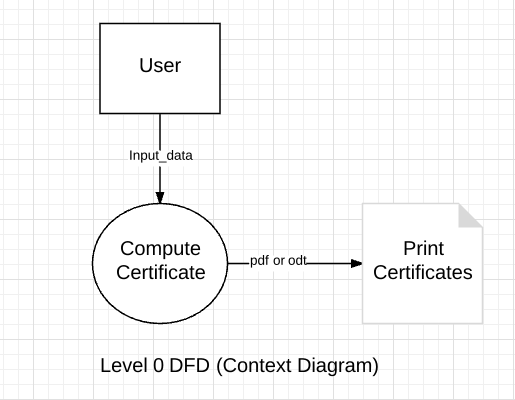
\includegraphics[scale=0.4]{images/cgs/dfd0.png}
\caption{Data flow LEVEL 0}
\label{fig:DFDs}
\end{figure}
Here, In figure \ref{fig:DFDs} figure \ref{fig:DF} and figure \ref{fig:DFd}
\begin{enumerate}
\item Institute details represent all initial input value
\item odt is the built-in file format in Ubuntu.
\item pdf is the portable document format.
\end{enumerate}
\begin{figure}
\centering 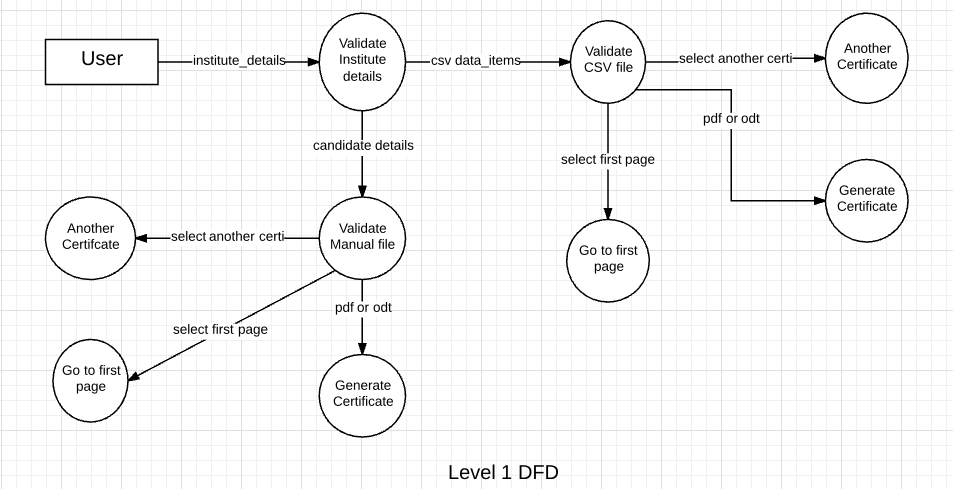
\includegraphics[scale=0.55]{images/cgs/dfd_1.png}
\caption{Data Flow LEVEL 1}
\label{fig:DF}
\end{figure}
\begin{figure}
\centering 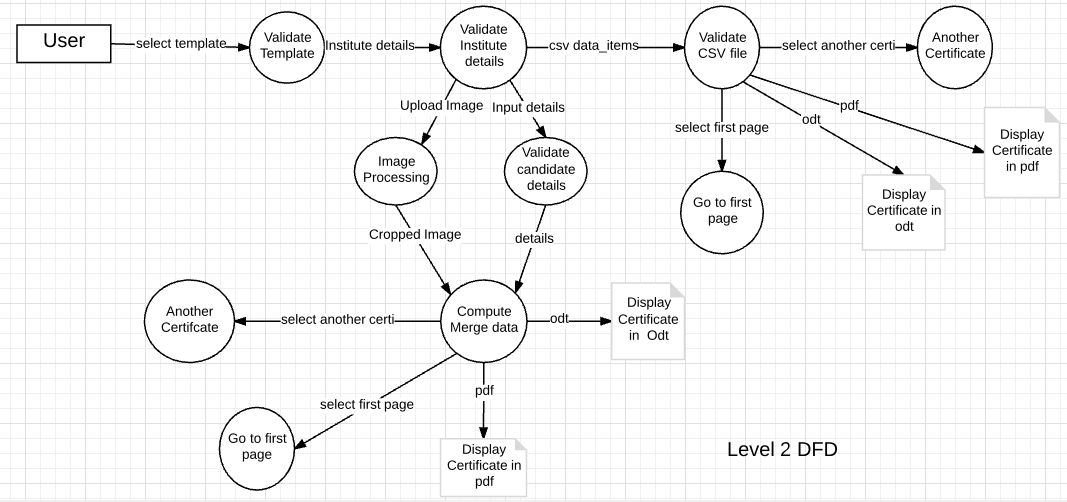
\includegraphics[scale=0.45]{images/cgs/dfd_2.png}
\caption{Data Flow LEVEL 2}
\label{fig:DFd}
\end{figure}

